\medskip

\textbf{Partie A}

\medskip



\begin{enumerate}
\item  La fonction dont la courbe représentative est la courbe $\mathcal{C}_{1}$ est décroissante sur $]-\infty~;~-2]$ et sur $[1~;~+\infty[$, et croissante sur $[-2~;~1]$.

La fonction dont la courbe représentative est la courbe $\mathcal{C}_{2}$ est négative sur

{$]-\infty~;~-2]$} et sur $[1~;~+\infty[$, et positive sur $[-2~;~1]$.

Les variations d'une fonction étant déterminées par le signe de sa dérivée, on peut en déduire que la courbe $\mathcal{C}_{1}$ est la courbe représentative de la fonction $g$ et la courbe $\mathcal{C}_{2}$ est la courbe représentative de la fonction $g'$. 


\item L'équation réduite de la tangente à la 
courbe représentative de la fonction $g$ au point d'abscisse 0 est : $y = g'(0)(x - 0)+ g(0)=g'(0)x+g(0)$.

La courbe $\mathcal{C}_{1}$ coupe l'axe des ordonnées au point de coordonnées $(0~;~1)$ donc $g(0)~=~1$.

La courbe $\mathcal{C}_{2}$ coupe l'axe des ordonnées au point de coordonnées $(0~;~2)$ donc $g'(0)~=~2$.

L'équation réduite de la tangente à la courbe représentative de la fonction $g$ au point d'abscisse 0 est donc $y = 2x+1$.
\end{enumerate}

\medskip

\textbf{Partie B}

\medskip



\begin{enumerate}
\item $f_{0}$ est dérivable sur $\R$ comme produit de fonctions dérivables sur $\R$. 

Pour tout réel $x$ :\quad 
$\begin{aligned}[t] f_0'(x) & = \left(2x+3\right) \times \e^{-x}+ \left(x^2+3x\right)\times (-\e^{-x})\\
	& = \left(2x+3-x^2-3x\right)\e^{-x}\\
	& =\left(-x^2-x+3\right)\e^{-x}
\end{aligned}$.

Pour tout réel $x$ on a donc :

$\begin{aligned} f_0(x)+f_0'(x)& = \left(x^{2}+3 x\right) \e^{-x}+\left(-x^2-x+3\right)\e^{-x}\\
	& = \left(x^{2}+3 x-x^2-x+3\right)\e^{-x}\\
	&=\left(2 x+3\right)\e^{-x}
\end{aligned}$ 

La fonction $f_{0}$  est une solution particulière de l'équation différentielle $(E)$.

	\item  $\left(E_{0}\right): y+y’=0 \iff y'=-y$ 

Les solutions sont donc les fonctions de la forme $x \longmapsto C\e^{-x}$, $C\in R$

	\item $(E)$ est une équation différentielle de la forme $y'=ay+f$, avec $f_0$ une solution particulière, les solutions sont donc les fonctions : \quad $x\longmapsto C\e^{-x } + f_0(x)$ avec $C\in\R$. (c'est à dire les fonctions $x\longmapsto  \left(x^{2}+3 x+C\right) \e^{-x} $  avec $C\in\R$.)
	\item La fonction $g$ décrite dans la \textbf{partie A} est une solution de l'équation différentielle $(E)$, il existe donc un réel $C$ tel que 
pour tout réel $x$, $g(x)= \left(x^{2}+3 x+C\right) \e^{-x} $. 

Or $g(0)=1$ donc $1=(0+0+C)\e^0=C$

L'expression de la fonction $g$ est donc : $g(x)= \left(x^{2}+3 x+1\right) \e^{-x} $. 
	\item La courbe admet exactement deux points d'inflexion si et seulement si la dérivée seconde de la fonction s'annule exactement deux fois en changeant de signe. 

Soit $f$ une solution de l'équation différentielle $(E)$. 

Il existe un réel $C$ tel que pour tout réel $x$, $f(x)= \left(x^{2}+3 x+C\right) \e^{-x}$. 

Déterminons la dérivée $f'$ et la dérivée seconde $f''$ de $f$. 

$\begin{aligned}
f'(x) & = \left(2x+3\right) \times \e^{-x}+ \left(x^2+3x+C\right)\times (-\e^{-x})\\
	& = \left(2x+3-x^2-3x-C\right)\e^{-x}\\
	& =\left(-x^2-x+3-C\right)\e^{-x}
\end{aligned}$.

et

$\begin{aligned}
f''(x) & = \left(-2x-1\right) \times \e^{-x}+ \left(-x^2-x+3-C\right)\times (-\e^{-x})\\
	& = \left(-2x-1+x^2+x-3+C\right)\e^{-x}\\
	& =\left(x^2-x-4+C\right)\e^{-x}
	\end{aligned}$.

Une fonction exponentielle est strictement positive sur $\R$ donc $f''(x)$ est du signe de $x^2-x-4-C$.

Un polynôme du second degré s'annule deux fois en changeant de signe  si et seulement si son discriminant est strictement positif.

Calculons le discriminant:

$\Delta = (-1)^2 -4 \times 1 \times (-4+C) = 1+16+4C=17-4C$

La courbe admettra donc exactement deux points d'inflexion si $17- 4C > 0$ c'est à dire $C < \dfrac{17}{4}$.

Les solutions de l'équation différentielle $(E)$ dont la courbe admet exactement deux points d'inflexion sont donc les fonctions de la forme :

$x\longmapsto \left(x^{2}+3 x+C\right) \e^{-x} $  avec $C<\dfrac{17}{4}$.
\end{enumerate}

\medskip

\textbf{Partie C}

\medskip







\begin{enumerate}
\item $f(x)=\left(x^{2}+3 x+2\right) \e^{-x} = \dfrac{x^2}{\e^x}+3 \dfrac{x}{\e^x} + \dfrac{2}{\e^x}$

$\lim\lim\limits_{x\to +\infty }\e^x= +\infty$ donc, par inverse, $\lim\limits_{x\to +\infty }\dfrac{1}{\e^x}=0$

Par croissances comparées : pour tout entier $n$ non nul, $\lim\limits_{x\to +\infty} \dfrac{x^n}{\e^x}= 0$
		
Donc par produit et par somme, $\lim\limits_{x \to +\infty} \dfrac{x^2}{\e^x}+3 \dfrac{x}{\e^x} + \dfrac{2}{\e^x} = 0$
\item 
	\begin{enumerate}
		\item Pour tout nombre réel $x$, 
$\begin{aligned}[t] f’(x)& =\left(2x+3\right) \e^{-x} + \left(x^2+3x+2\right)\left(-\e^{-x}\right)\\
	& = \left( 2x+3-x^2-3x-2\right)\e^{-x}\\
	& = \left(-x^2-x+1\right)\e^{-x}
\end{aligned}$.
\item Une fonction exponentielle est strictement positive sur $\R$ donc $f'(x)$ est du signe du polynôme du second degré $-x^2-x-1$. 

$\Delta=(-1)^2-4 \times (-1)\times 1= 1+4=5>0$

Le polynôme admet donc deux racines : 

$x_1= \dfrac{1+\sqrt{5}}{-2}= \dfrac{-1-\sqrt{5}}{2}$ \quad et \quad $x_2= \dfrac{1-\sqrt{5}}{-2}= \dfrac{-1+\sqrt{5}}{2}$

Le coefficient dominant est positif on en déduit donc :




\begin{tikzpicture}
\tkzTabInit[lgt=2.2,espcl=3]{$x$/0.7,
signe de $f'(x)$/0.7,
variations de $f$/2}{$-\infty$,$x_1$,$x_2$,$+\infty$}
\tkzTabLine{,-,z,+,z,-,}
\tkzTabVar{+/$+\infty$,-/$f(x_1)$,+/$f(x_2)$,-/$0$}
\end{tikzpicture}\hfill~

La fonction $f$ est décroissante sur $\left] -\infty~;~\dfrac{-1-\sqrt{5}}{2}\right[$ et sur $\left] \dfrac{-1+\sqrt{5}}{2}~;~ +\infty \right[$.

Elle est croissante sur $\left]\dfrac{-1-\sqrt{5}}{2}~;~\dfrac{-1+\sqrt{5}}{2}\right[$.
	\end{enumerate}
\item Une fonction exponentielle est strictement positive sur $\R$ donc $f(x)$ est du signe du polynôme du second degré $x^2 + 3x + 2$.

Pour tout réel $x$ : $x^2+3x+2 =(x+2)(x+1)$ 

Les racines sont donc $-2$ et $-1$.

De plus le coefficient dominant est positif donc $x^2+3x+2$ est positif, entre autre, sur l'intervalle $]-1~;~ +\infty[$ et donc sur l'intervalle $[0~;~+\infty[$.

La fonction $f$ est donc positive sur l'intervalle $[0~;~+\infty[$.

\item La fonction $f$ est positive sur l'intervalle $[0;+\infty[$ donc sur $[0~;~\alpha]$ donc l'aire $\mathcal{A}(\alpha)$, exprimée en unité d'aire, du domaine du plan délimité par l'axe des abscisses, la courbe $\mathcal{C}_{f}$ et les droites d'équation $x=0$ et $x=\alpha$ est égale à $\displaystyle  \int_0^{\alpha}f(x) \,\rm{d} x$.

$\begin{aligned} \mathcal{A}(\alpha) & = \displaystyle  \int_0^{\alpha}f(x) \,\rm{d} x\\
	& = {\left[ F(x) \right]}_0^{\alpha}\\
	& = F(\alpha)-F(0)\\
	&= \left( -\alpha^2-5\alpha-7\right)\e^{-\alpha}+ 7
\end{aligned}$

L'aire cherchée est égale à $ \left( -\alpha^2-5\alpha-7\right)\e^{-\alpha}+7$ unités d'aire.

\end{enumerate}
